\documentclass[parskip=full, a4paper]{scrreprt}

%%% PACKAGES %%%

% add unicode support and use german as language
\usepackage[utf8]{inputenc}
\usepackage[ngerman]{babel}

% Use Helvetica as font
\usepackage[scaled]{helvet}
\renewcommand\familydefault{\sfdefault}
\usepackage[T1]{fontenc}

% Better tables
\usepackage{tabularx}

% Better enumerisation env
\usepackage{enumitem}

% Use graphics
\usepackage{graphicx}

% Have subfigures and captions
\usepackage{subcaption}

% Be able to include PDFs in the file
\usepackage{pdfpages}

% Have custom abstract heading
\usepackage{abstract}

% Need a list of equation
\usepackage{tocloft}
\usepackage{ragged2e}

% Better equation environment
\usepackage{amsmath}

% Symbols for most SI units
\usepackage{siunitx}

\usepackage{csquotes}

% Clickable Links to Websites and chapters
\usepackage{hyperref}

% Change page rotation
\usepackage{pdflscape}

% Symbols like checkmark
\usepackage{amssymb}
\usepackage{pifont}

\usepackage[absolute]{textpos}

% Glossary, hyperref, babel, polyglossia, inputenc, fontenc must be loaded before this package if they are used
\usepackage{glossaries}
% Redefine the quote charachter as we are using ngerman
\GlsSetQuote{+}
% Define the usage of an acronym, Abbreviation (Abbr.), next usage: The Abbr. of ...
\setacronymstyle{long-short}
\makeglossaries

% Bibliography & citing
\usepackage[
backend=biber,
style=apa,
bibstyle=apa,
citestyle=apa,
sortlocale=de_DE
]{biblatex}
\addbibresource{Referenzen.bib}
\DeclareLanguageMapping{ngerman}{ngerman-apa}

%%% TOC Header
\addto\captionsngerman{
	\renewcommand{\contentsname}{Traktanden}
}

%%% Not clearpage before chapter
\usepackage{etoolbox}
\makeatletter
\patchcmd{\scr@startchapter}{\if@openright\cleardoublepage\else\clearpage\fi}{}{}{}
\makeatother

%%% Fallback DocumentVersion if Builded local
\providecommand{\docversion}{0.0-localBuild}

%%% DOCUMENT %%%

\begin{document}
\begin{titlepage}
\vspace*{2.5cm}
\noindent
\Huge{\textbf{Sitzungsprotokoll SprintReview}} \\
\noindent
\Large{15.05.2019, Rotkreuz}\\
\vfill
\noindent
\large{Author: Dane Wicki}\\
\noindent
\large{Datum: \today}\\
\noindent
\large{Version: \docversion}\\
\end{titlepage}

\noindent
\begin{tabularx}{\textwidth}{XXl}
\hline \\
\multicolumn{3}{l}{\Large{\textbf{SprintReview  Bachelorarbeit}}}\\
\multicolumn{3}{l}{Suche von mit RFID ausgerüsteten Einzelexemplaren} \\ \\
\hline
	Freitag, & & Hochschule Luzern \\
	15. Mai 2019 & 08:00 Uhr bis 09:30 Uhr & Raum 41.411, Rotkreuz \\
\hline \\
\hline
Besprechungsart & SprintReview & \\
\hline
Besprechungsleiter & Pascal Baumann & \\
\hline
Protokollführer & Dane Wicki & \\
\hline
Teilnehmer & Mike Märki & \\ & Pascal Baumann & \\ & Dane Wicki & \\
\hline
Teilanwesend & Prof. Martin Jud & \\
\hline
\end{tabularx}

	\noindent

\tableofcontents
\clearpage
\chapter{Versuchsdurchführung}
Herr Wicki führte auf, dass bei der letzten Durchführung lediglich ein Bericht an Herr Märki gesendet wird, welcher die Versuche zusammenfasst.
Weiter entschuldigte er sich für die kleine Verspätung dieser Abgabe, diese sei dadurch zu erklären durch die etwas verspätete Ankunft der RFID Hardware, da diese zu diesem Zeitpunkt von den Studierenden bezahlt werden musste.

Anschliessend ging Herr Wicki einen ersten Versuch ein, bei welchem es um das Bulk Reading ging. Dieser wurde ausgewählt für die Besprechung, da es ein wichtiger Bestandteil beider Konzepte ist, da es in einem Behälter jeweils viele Exemplare hat. Herr Wicki führte auf, dass bei diesem Versuch auf einer Hölzernen Halterung montiert wurde, und darunter sich die zu lesenden Tags befinden (siehe Abbildung \ref{fig:positionTagsForBulkreading}).
\begin{figure}[htb]
	\centering
	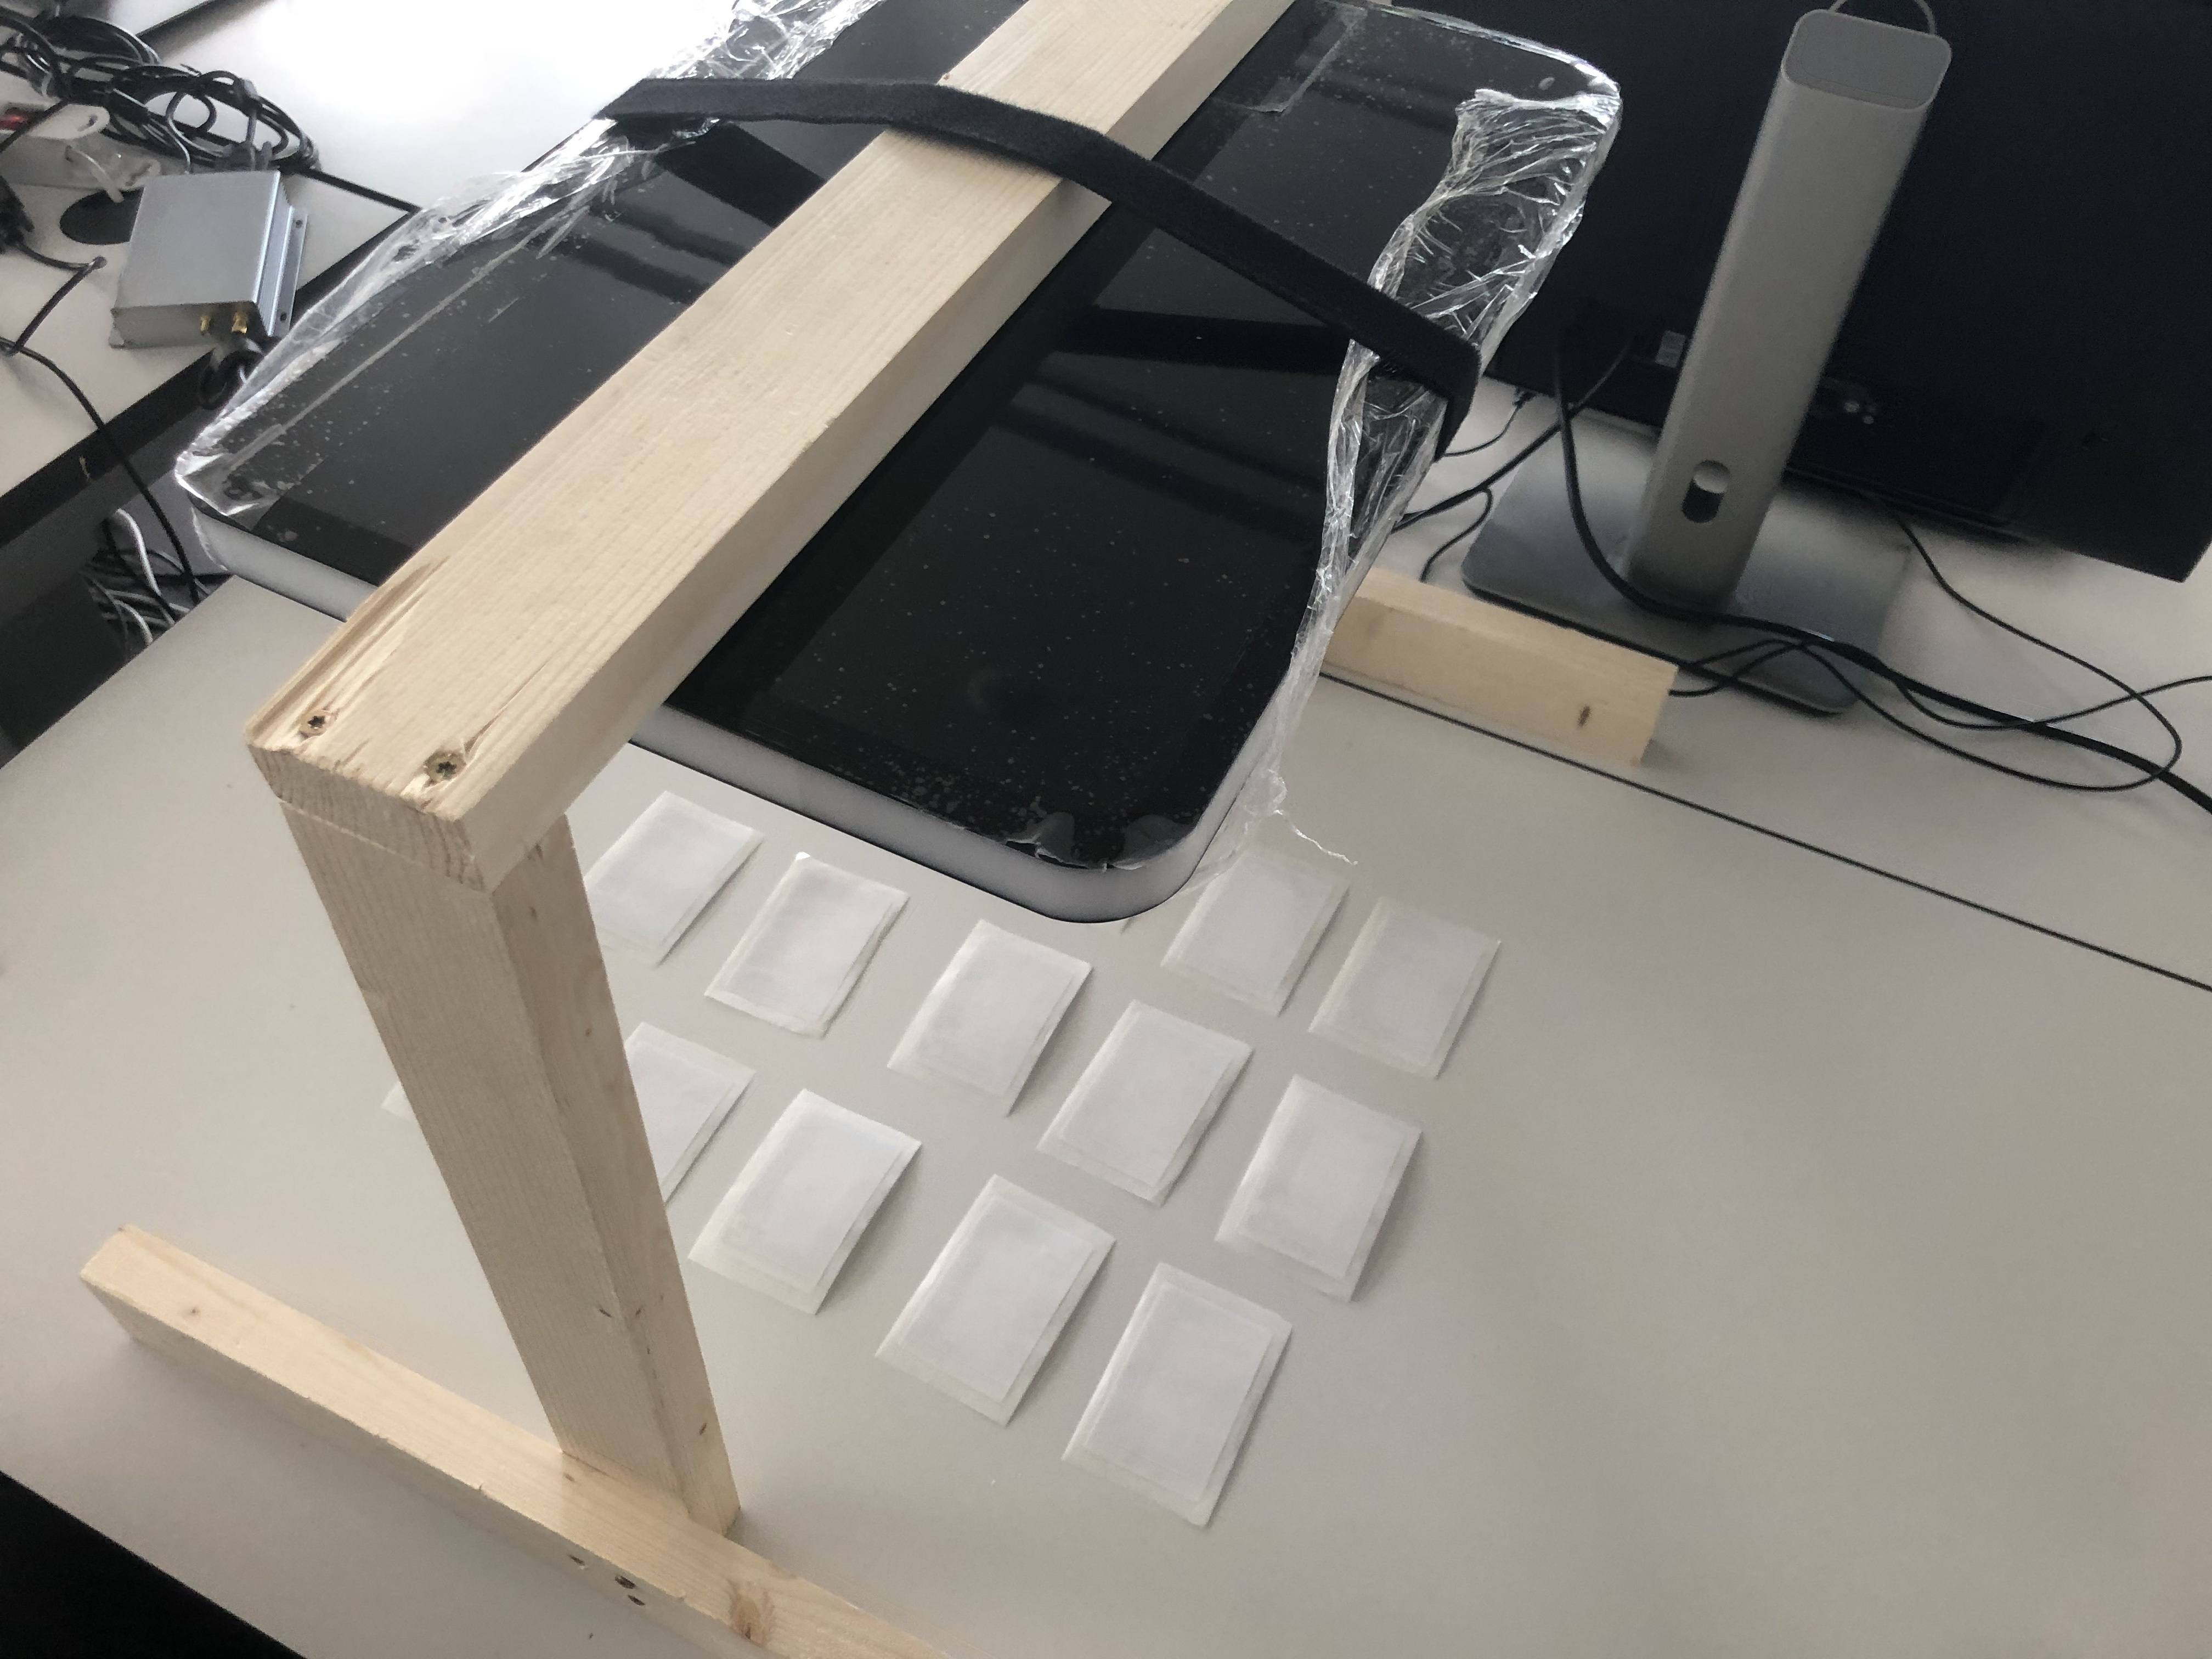
\includegraphics[keepaspectratio,width=.7\linewidth]{img/PositionTagsBulkreading}
	\caption{Tag positionierung für Bulk Reading}
	\label{fig:positionTagsForBulkreading}
\end{figure}
Herr Wicki führt auf, dass bei diesem Versuch schnell herausgefunden werden konnte, dass die seitliche Distanz der Tags zueinander auch Auswirkungen auf Lesbarkeit hat. Herr Märki fragte nach, ob sich diese Lesbarkeit verschlechtert, darauf führte Herr Wicki an, dass es ab einer Distanz gar nicht mehr geht und keine Verschlechterung stattfindet, sondern dass nur noch ein Tag von mehreren antwortet. Herr Märki fragte anschliessend nach, ob es sich beim Bulk Reading um das Auslesen aller vorhandenen Tags handelt. Herr Wicki bestätigte dies. Herr Märki fragte nochmals nach, ob die Tags trotz der Nähe eine auswertbare Antwort liefer. Herr Wicki entgegnete, dass sobald die Tags einen kritischen Punkt überschreiten und zu nahe aneinander liegen, die Tags keine auswertbare Antwort liefern. Herr Wicki führte weiter an, dass der Fall, dass die Tags auf derselben Achse zu nahe aneinanderliegen bei eingelagerten Exemplaren eher unwahrscheinlich sein sollte, da die Tags meist nicht unmittelbar am Rande eines Buches angeklebt anzutreffen sind. Herr Wicki zeigte anhand der vorhandenen Tags und einem Buch, wie gross der Abstand der Tags zwischen den Büchern ist. Herr Märki fügte an, dass die Tags, welche Herr Wicki und Herr Baumann verwenden etwas grösser seien, als diejenigen, welche bei der Speicherbibliothek vorhanden sind. Herr Wicki fügte jedoch an, dass es sich bei den vorhandenen Tags um reale Tags, welche von der ZHB zur Verfügung gestellt wurden, handelt. Herr Baumann zeigte anschliessend anhand des Buches, wie die Bücher platziert sind, und der Abstand der Bücherreihen zueinander gross genug sein sollten. Herr Wicki fügte noch an, dass es sich bei diesem Versuch nicht um den Abstand von gestapelten Tags handle, sondern um auf einer Ebene befindliche Tags, welche jeweils zueinander Abstand halten müssen.
Herr Baumann fügte noch an, dass mit diesem Versuch primär die Lesezeit, sowie die maximale Anzahl lesbarer Tags ermittelt werden sollten. Weiter fügte er an, dass, wie im Testprotokoll zu entnehmen ist, die Lesezeit mit zunehmender Anzahl zu lesenden Tags, zunimmt. Er fügte anschliessend noch hinzu, dass bei einer Gesamtanzahl von 15 Tags keine Weiteren hinzugefügt wurden, Herr Wicki begründete dies, dadurch, dass das Fernbleiben weiterer Tags durch die Aufbauvorrichtung zu verschulden ist, welche es nicht zuliess, weitere Tags an der Seite zu platzieren.

Herr Märki fragte anschliessend ob nur ein einzelner bestimmter Tag gesucht werden kann und ob zwei bereits schwieriger ist zu realisieren. Herr Wicki entgegnete, dass es sich bei diesem Test um ein Bulk Reading handelte, welches ausschliesslich im Konzept 2 zum Tragen kommt. Weiter führte er auf, dass beim Bulk Reading einfach alle Tags gesucht und inventarisiert werden, welche erreichbar sind.
Herr Baumann merkte weiter an, dass das spezifische Abfragen nach einem einzelnen Tag in einem anderen Versuch untersucht wurde. Bei diesem würde einfach abgefragt, ob ein Tag mit einer bekannten Tag-ID vorhanden ist und dieser würde, sofern dieser erreichbar ist, antworten.

Herr Wicki rekapitulierte, dass mit dem Versuch des Bulk Reading die Erkenntnis gewonnen werden konnte, dass die Tags auch auf einer Ebene einen gewissen Mindestabstand zueinander haben müssen.
Anschliessend fuhr Herr Wicki zum Versuch der seitlichen Reichweite fort. Er fügte an, dass dieser Versuch insofern interessant ist, dass mit diesem Versuch überprüft werden kann, ob auch die gesamte Breite eines Behälters ausgelesen werden kann.
Herr Märki fragte nach, ob es bei diesem Versuch auch um die Ausrichtung der Antenne und dem Tag hier überprüft wird. Herr Wicki verwies darauf hin, dass dies in einem späteren Versuch überprüft wurde.
Herr Wicki fuhr anschliessend mit den Resultaten des Versuches fort anhand eines Graphen, welches die Reichweite sowie die seitliche Reichweite festhält (siehe Abbildung \ref{fig:abdeckungSeitlicheReichweite}).
\begin{figure}[htb]
	\centering
	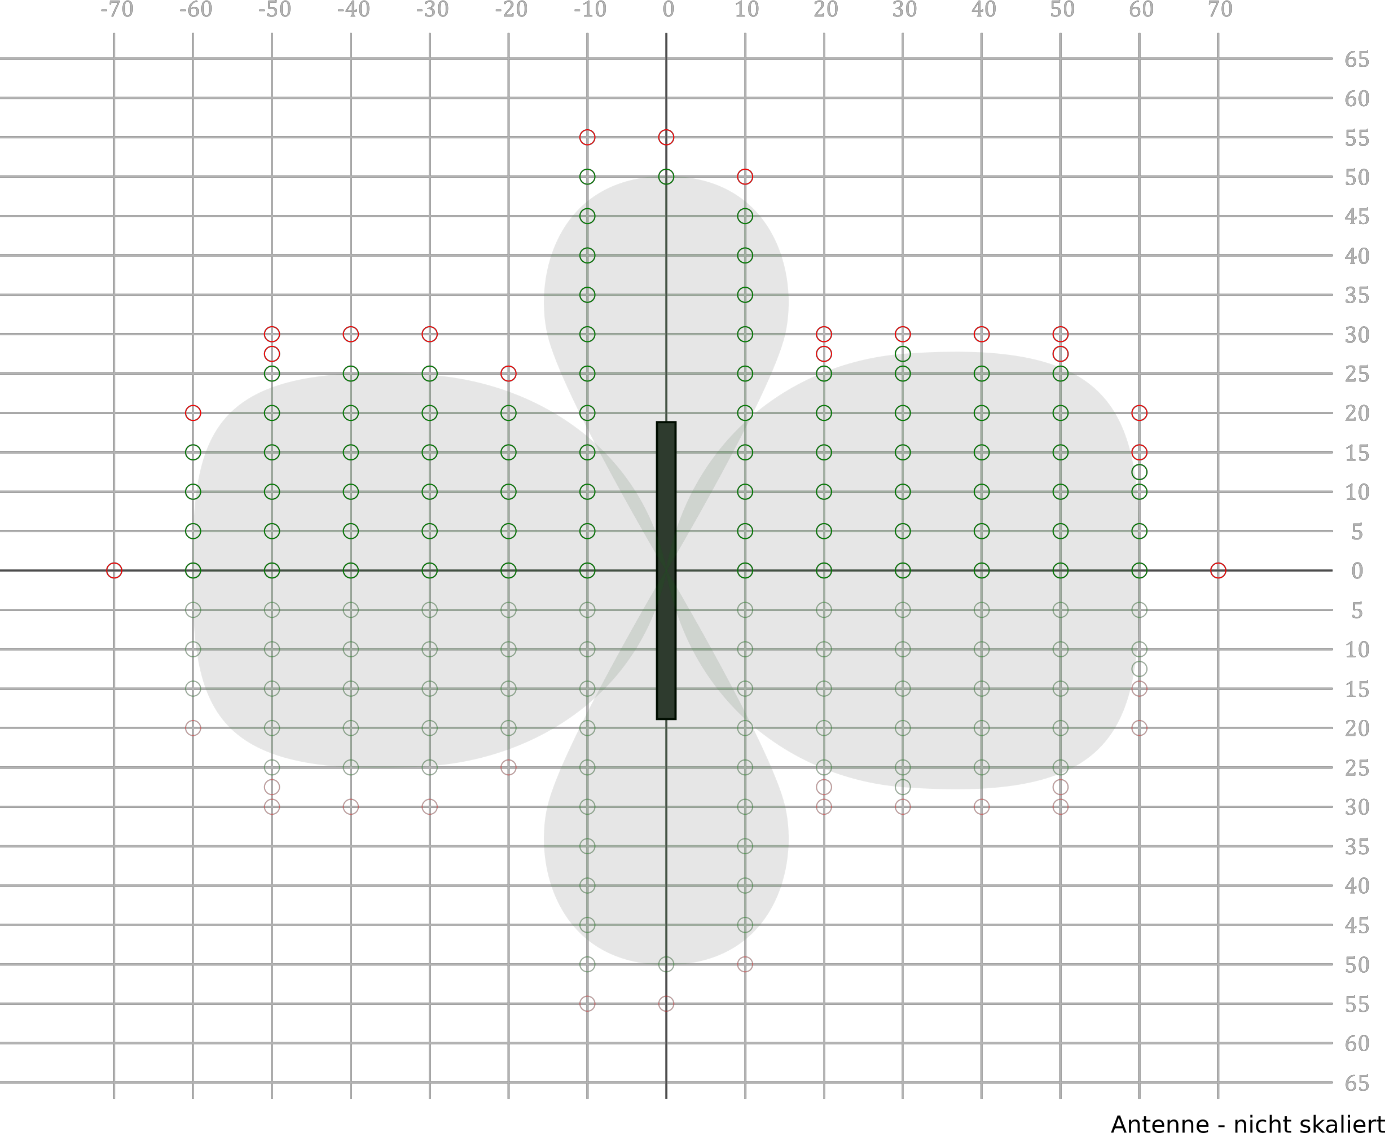
\includegraphics[keepaspectratio,width=\linewidth]{img/seitlicheReichweiteVersuch}
	\caption{Resultate der Leseabdeckung bei seitlicher Reichweite}
	\label{fig:abdeckungSeitlicheReichweite}
\end{figure}
Herr Wicki fuhr fort, dass es ziemlich interessant war, da mit diesem Versuch bekannt wurde, dass die verwendete Antenne nach vorne, wie auch nach hinten lesen kann. Zudem ist es interessant zu wissen, dass die verwendete Antenne auch auf der Seite nochmals einen stärkeren Ausschlag aufweist als angenommen. Herr Wicki erklärte, dass der auf der Grafik abgebildete Schwarze Balken die Antenne darstellen sollte. Zudem erklärte er die Ausrichtung anhand der im Sitzungszimmer vor Ort vorhandenen Antenne.
Weiter fuhr Herr Wicki fort, dass die Erkenntnisse dahingehend sehr hilfreich sind, als dass diese schon Hinweise für potenzielle Abschirmungen liefern.
So muss die Antenne, sofern das Potenzial besteht, dass sich Exemplare auch direkt dahinter befinden, gegen diese Bereiche mittels Metallplatten abgeschirmt werden.

Herr Wicki fuhr weiter mit dem nächsten Test, bei welchem es um verschiedene Möglichkeiten der Abschirmung geht. Herr Wicki wies darauf hin, dass Störobjekte wie etwa Plastik, Bücher und Metall in diesem Versuch getestet wurden. Daraufhin erklärte Herr Wicki, dass der Versuch mit 7 Büchern und dem Behälter durchgeführt wurden, bei welchem der Tag hinter 2 Behälterwänden und dazwischen noch 7 Bücher platziert wurde (siehe Abbildung \ref{fig:bucherMitBehälterAlsAbschirmung}). Er fasste kurz zusammen, dass in Verbindung mit den Büchern und dem Behälter keine Beeinträchtigungen festgestellt werden konnten.

\begin{figure}[htb]
	\centering
	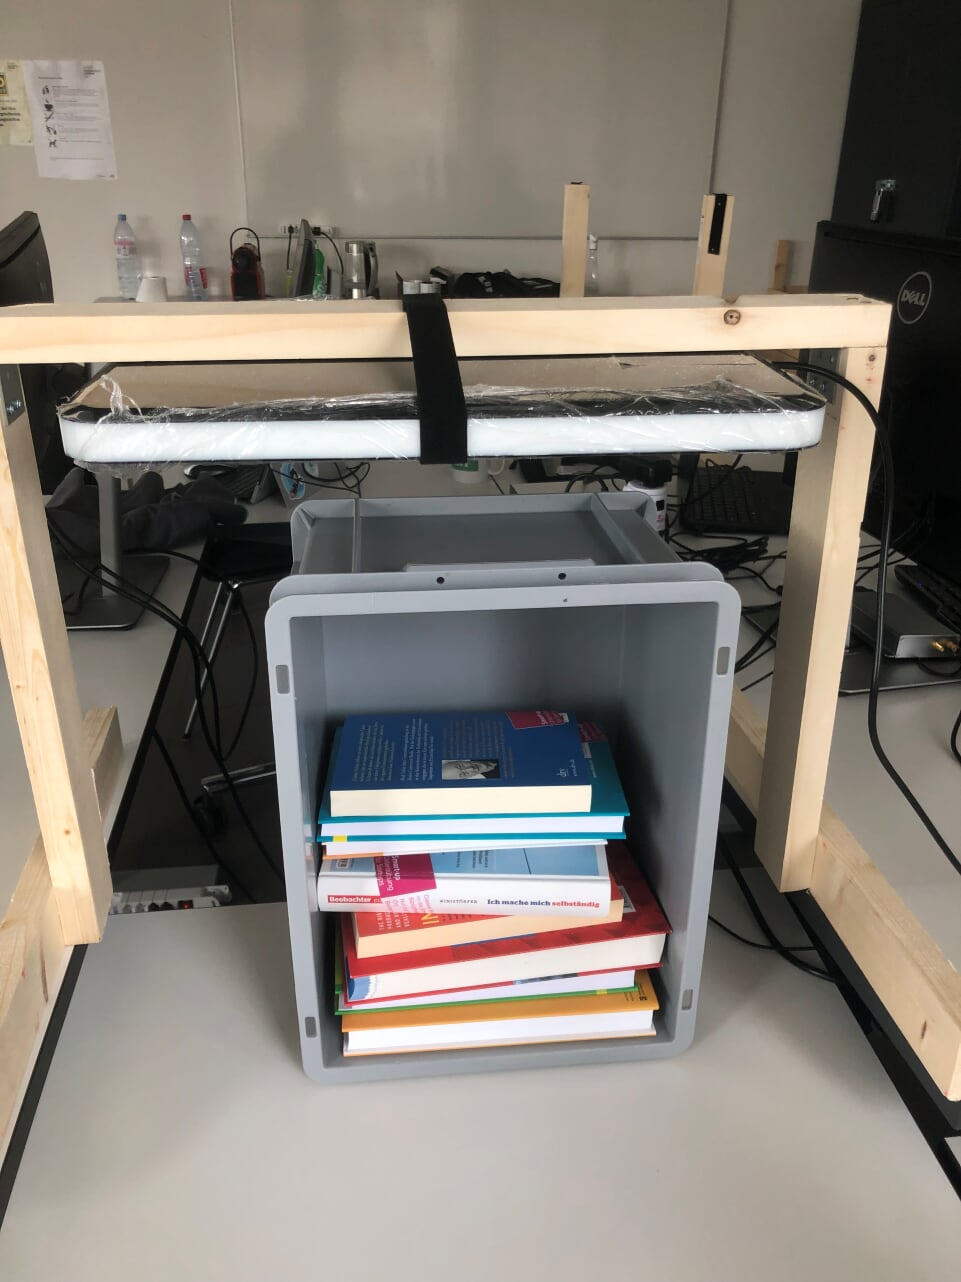
\includegraphics[keepaspectratio,width=.6\linewidth]{img/AbschirmungDurchBehaelter}
	\caption{Abschirmung des Tags durch Behälter und Bücher}
	\label{fig:bucherMitBehälterAlsAbschirmung}
\end{figure}

Herr Wicki führte fort mit der Aussage, dass die Versuche aufzeigten, dass bereits bei sehr dünnen Metallplatten (Aluminium und Stahl wurden verwendet) eine Abschirmung von 100\% erreicht werden konnte. Weiter fügte er an, dass dies eine Verunmöglichung des Konzept Eins darstellt, welches im Hochregallager nach einem deplatzierten Exemplar suchen würde.
Herr Märki merkte an, dass es trotzdem noch funktionieren könnte, indem man nur noch die benachbarten Behälter auf derselben Höhe auslesen würde. Herr Wicki wie auch Herr Baumann bestätigten, dass dies theoretisch noch möglich sei, jedoch nicht mit dieser Hardware, da diese eine maximale Lesereichweite von 60cm aufweist und der Behälter bereits 60cm ist und es bei einer Messung vom Roboter noch einen gewissen Abstand zum Lager besteht. Herr Märki fragte anschliessend ob das Konzept mit der Suche im Hochregallager noch nicht verworfen ist. Herr Wicki antwortete, mit der Aussage, dass mit der verfügbaren Hardware die Suche im Hochregallager keine Option mehr ist und daher von Herr Wicki und Herr Baumann nicht weiter untersucht werden kann, da keine zufriedenstellende Aussage getätigt werden könnte.

Herr Wicki fuhr weiter mit einer kurzen Zusammenfassung aller Störquellenversuche, bei welcher die Kernaussage war, dass ausser Metall keine weiteren Störquellen gefunden werden konnten.

Anschliessend fuhr Herr Wicki mit dem Versuch von gestapelten Tags fort. Bei diesem Versuch konnte, gemäss Herr Wicki, festgestellt werden, dass ein Mindestabstand von 3cm zwischen zwei aufeinanderliegenden Tags genügen, damit sich diese nicht weiter stören können. Als Fazit fügte er noch an, dass dieses Problem nur solange besteht, wie die Tags passend aufeinanderliegend, sobald diese jedoch um wenige Zentimeter versetzt sind, diese wieder in einem Abstand von circa einem Zentimeter gelesen werden können.
Herr Wicki beschrieb kurz, wie der Versuch durchgeführt wurde. Anschliessend schloss Herr Wicki diesen Versuch mit dem Fazit ab, dass nicht alle Tags gelesen werden könnte, sofern es Exemplare enthält, welche nur sehr schmal sind.
Herr Märki fragte, ob dieses Problem nur bei einem Bulk Reading oder auch bei der Einzelexemplarsuche besteht. Herr Baumann erwiderte, dass es sich hierbei um den Bulk Reading Modus handelt. Herr Wicki erwiderte zusätzlich noch, dass zu diesem Zeitpunk das Konzept mit der Suche nach einem Einzelexemplar im Hochregallager zu diesem Zeitpunkt mit dieser Hardware bereits verworfen werden musste, da die Distanz von über 80cm für dieses Konzept nicht erreicht werden kann, sowie die Dicke der Antenne keinen Einsatz mehrere Antennen in einem Behälter zulässt.
Herr Märki erwiderte auf die Bemerkung von Herr Wicki, dass die Einzelexemplarsuche jedoch auch für das Konzept mit der Erstellung eines Arbeitsprozesses eingesetzt werden könnte.
Es folgte eine kurze Diskussion zum Obsoleten Thema der Einzelsuche (Obsolet, da Einzelexemplarsuche das Wissen der Tag-ID als Voraussetzung gibt, dies jedoch nicht gegeben ist, siehe Kapitel \ref{result:noSingleTagReachable}).

Herr Wicki schloss die Präsentation der Versuche mit dem Versuch der Ausrichtung der Antennen ab. Herr Baumann erklärte kurz, dass bei Ausrichtungen ab ca. 60\SIUnitSymbolDegree die Tags wieder Lesbar sind (Nachtrag, ein weiterer Versuch hat aufgezeigt, dass auch 90\SIUnitSymbolDegree gelesen werden kann, sofern der Tag sich ca. 20cm Seitlich des Antennenmittelpunktes befindet, was bei dem bewegenden Behälter gegeben ist).

Herr Wicki schloss die Versuche mit dem Fazit ab, dass das Konzept Zwei für die Machbarkeitsstudie verwendet wurde. Zudem wurden für dieses Konzept Anpassungen vorgenommen, um Tags auch besser Winkel-unabhängig auszulesen. Herr Wicki führte zudem noch auf, dass das Konzept so angepasst wurde, dass die Behälter gelesen werden können, welche gemäss Abbildung \ref{fig:behaelterFuellung} befüllt sind.
\begin{figure}[htb]
	\begin{subfigure}{.6\linewidth}
		\centering
		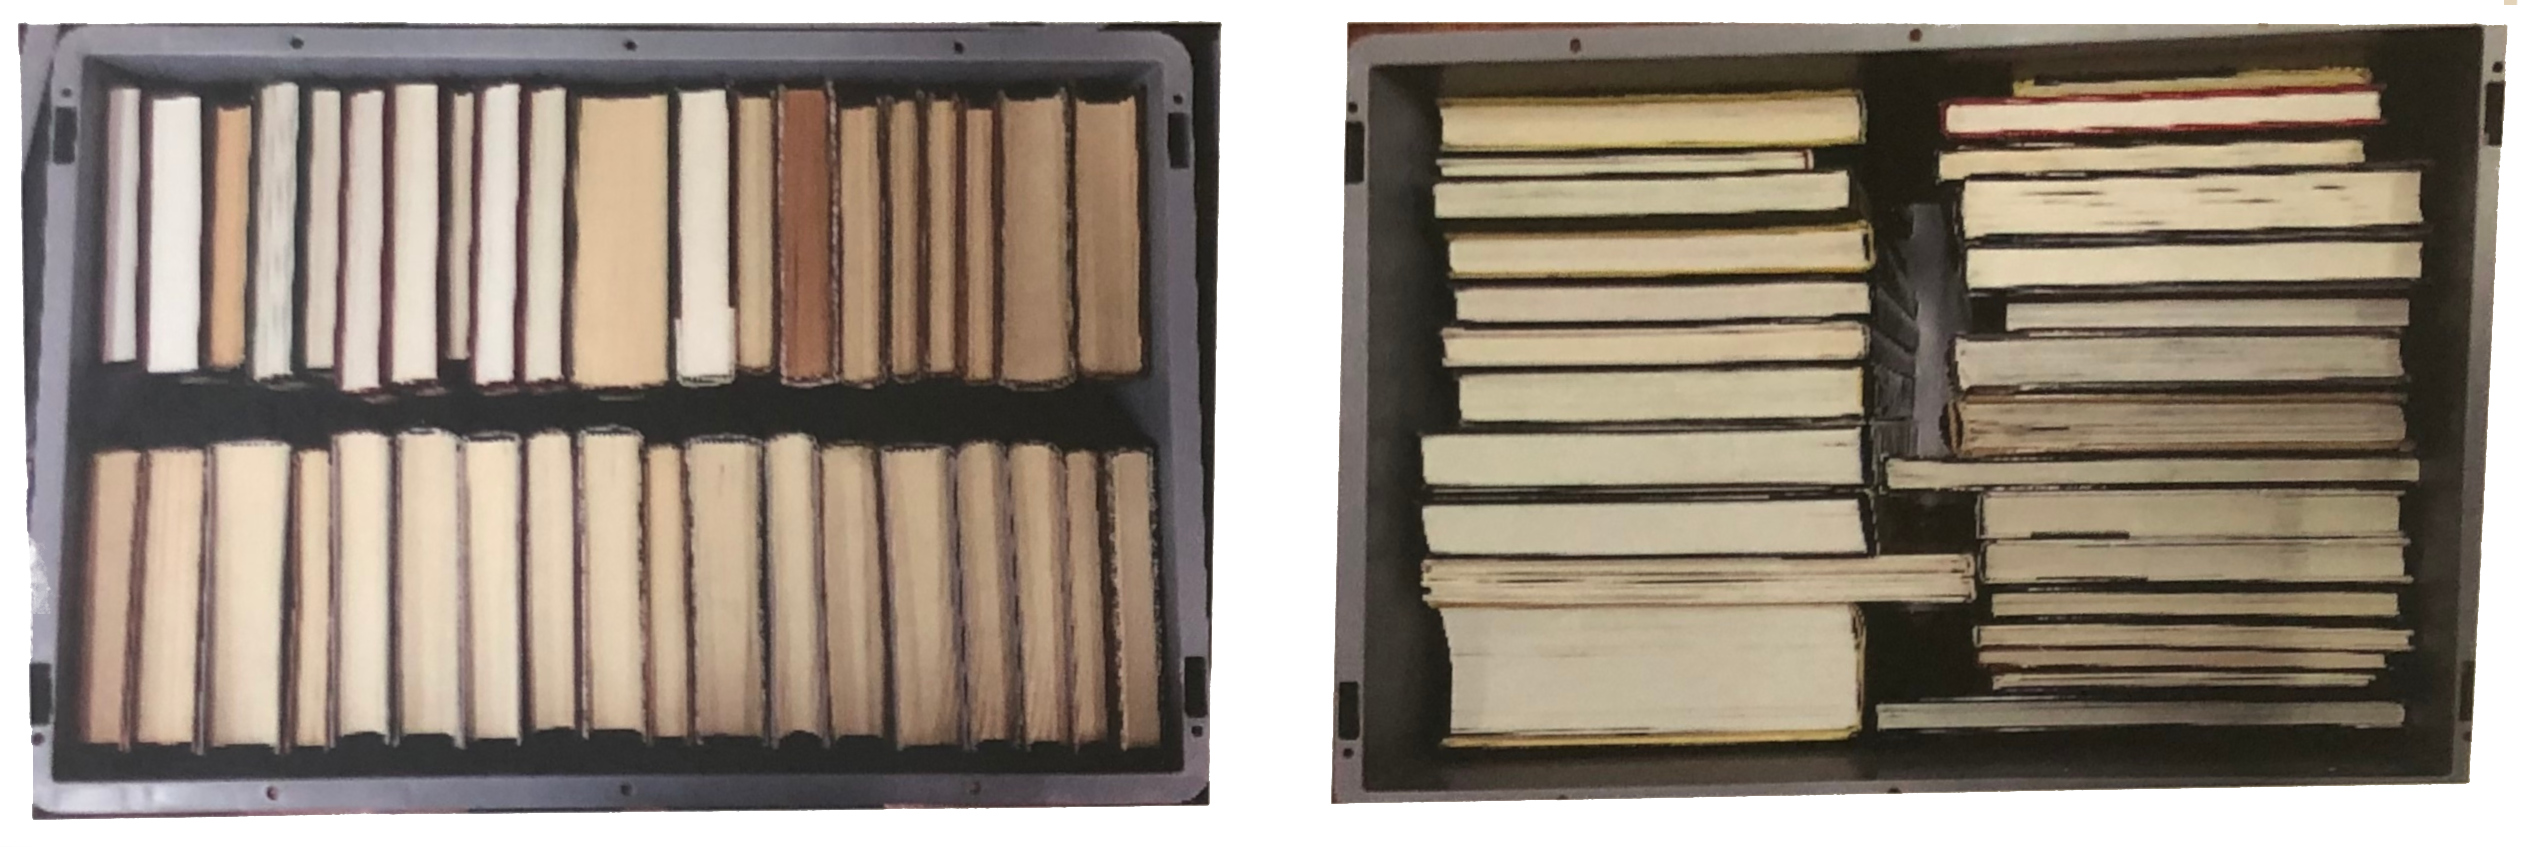
\includegraphics[keepaspectratio,height=3cm]{img/LagerungExemplare}
		\caption{Lesbare Lagerungsarten}
		\label{fig:behaelterFuellung}
	\end{subfigure}
	\begin{subfigure}{.4\linewidth}
		\centering
		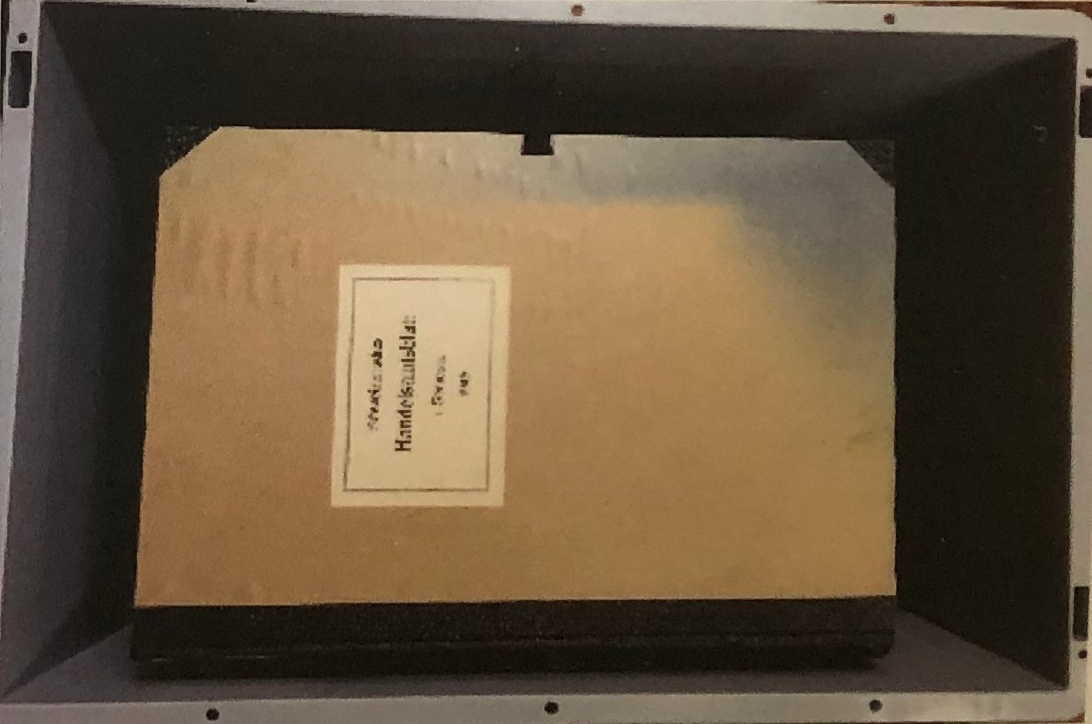
\includegraphics[keepaspectratio,height=2.9cm]{img/LagerungExemplareNichtLesbar}
		\caption{Nicht lesbare Lagerungsarten}
		\label{fig:behaelterFuellungNichtLesbar}
	\end{subfigure}
	\caption{Lagerungsarten}
\end{figure}
Exemplare, welche gemäss Abbildung \ref{fig:behaelterFuellungNichtLesbar} befüllt werden, sind nicht lesbar. Herr Märki fügte an, dass es sich bei den nicht lesbaren Behälter um Blätter oder auch alte Zeitungen handeln kann. Weiter fügte er an, dass um diesen Behälter lesen zu können noch eine dritte Antenne eingesetzt werden könnte. Herr Wicki bestätigte dies unter dem Vorbehalt, dass dies jedoch mit der jetzigen Hardware nicht testbar ist und dadurch nicht ins Konzept eingeflossen ist, dies jedoch durchaus eine Option für die Betrachtung sei. Herr Wicki fragte jedoch noch kurz nach, ob diese Lagerungsposition häufig zum Einsatz kommt. Herr Märki antwortete mit der Aussage, dass dies nicht der Fall sei. Herr Wicki erwiderte, dass sofern diese Lagerungsmöglichkeit wirklich nicht zu häufig anzutreffen ist, die Gefahr des deplatzieren noch geringer vorhanden ist als bei den anderen Behälter und daher dies doch vernachlässigbar sei. Es gab keine Einwände gegen diese Aussage.

\chapter{Machbarkeitsstudie}
Herr Baumann fasste kurz zusammen, dass die Machbarkeitsstudie stark an die Struktur eines Dokumentes des Departement of Agriculture aus Amerika angelehnt ist. Zudem ist die Machbarkeitsstudie sehr stark wirtschaftlich fokussiert. Herr Baumann führte fort, dass das erste Kapitel sicherlich das interessanteste ist, da sich dort die Entscheidung wie auch die Empfehlung befinden. Er führte zudem auf, dass in der Machbarkeitsstudie auf Feig Electronic gesetzt wurde, da damit eine höhere Reichweite erreicht werden kann. Herr Märki fragte kurz nach, weshalb eine höhere Reichweite gewünscht ist. Herr Wicki beantwortete, dass mit der Anpassung der Machbarkeitsstudie eine neue Antenne hinzugestossen ist, welche die erhöhte Reichweite gut gebrauchen kann. Er führte zudem auf, dass für die neue Position die Antenne Schräg am Rande (siehe Abbildung \ref{fig:antenneSchraeg}) positioniert wurde mit einer Abschirmung zum weiteren Förderband. Herr Wicki fuhr fort, dabei begründete er, dass Feig zu empfehlen sei, da diese bereits von führenden Lösungsanbietern wie Bibliotheka verwendet werden, wie auch der Tatsache, dass die Speicherbibliothek bereits Feig Hardware im Einsatz hat.

\begin{figure}[htb]
	\centering
	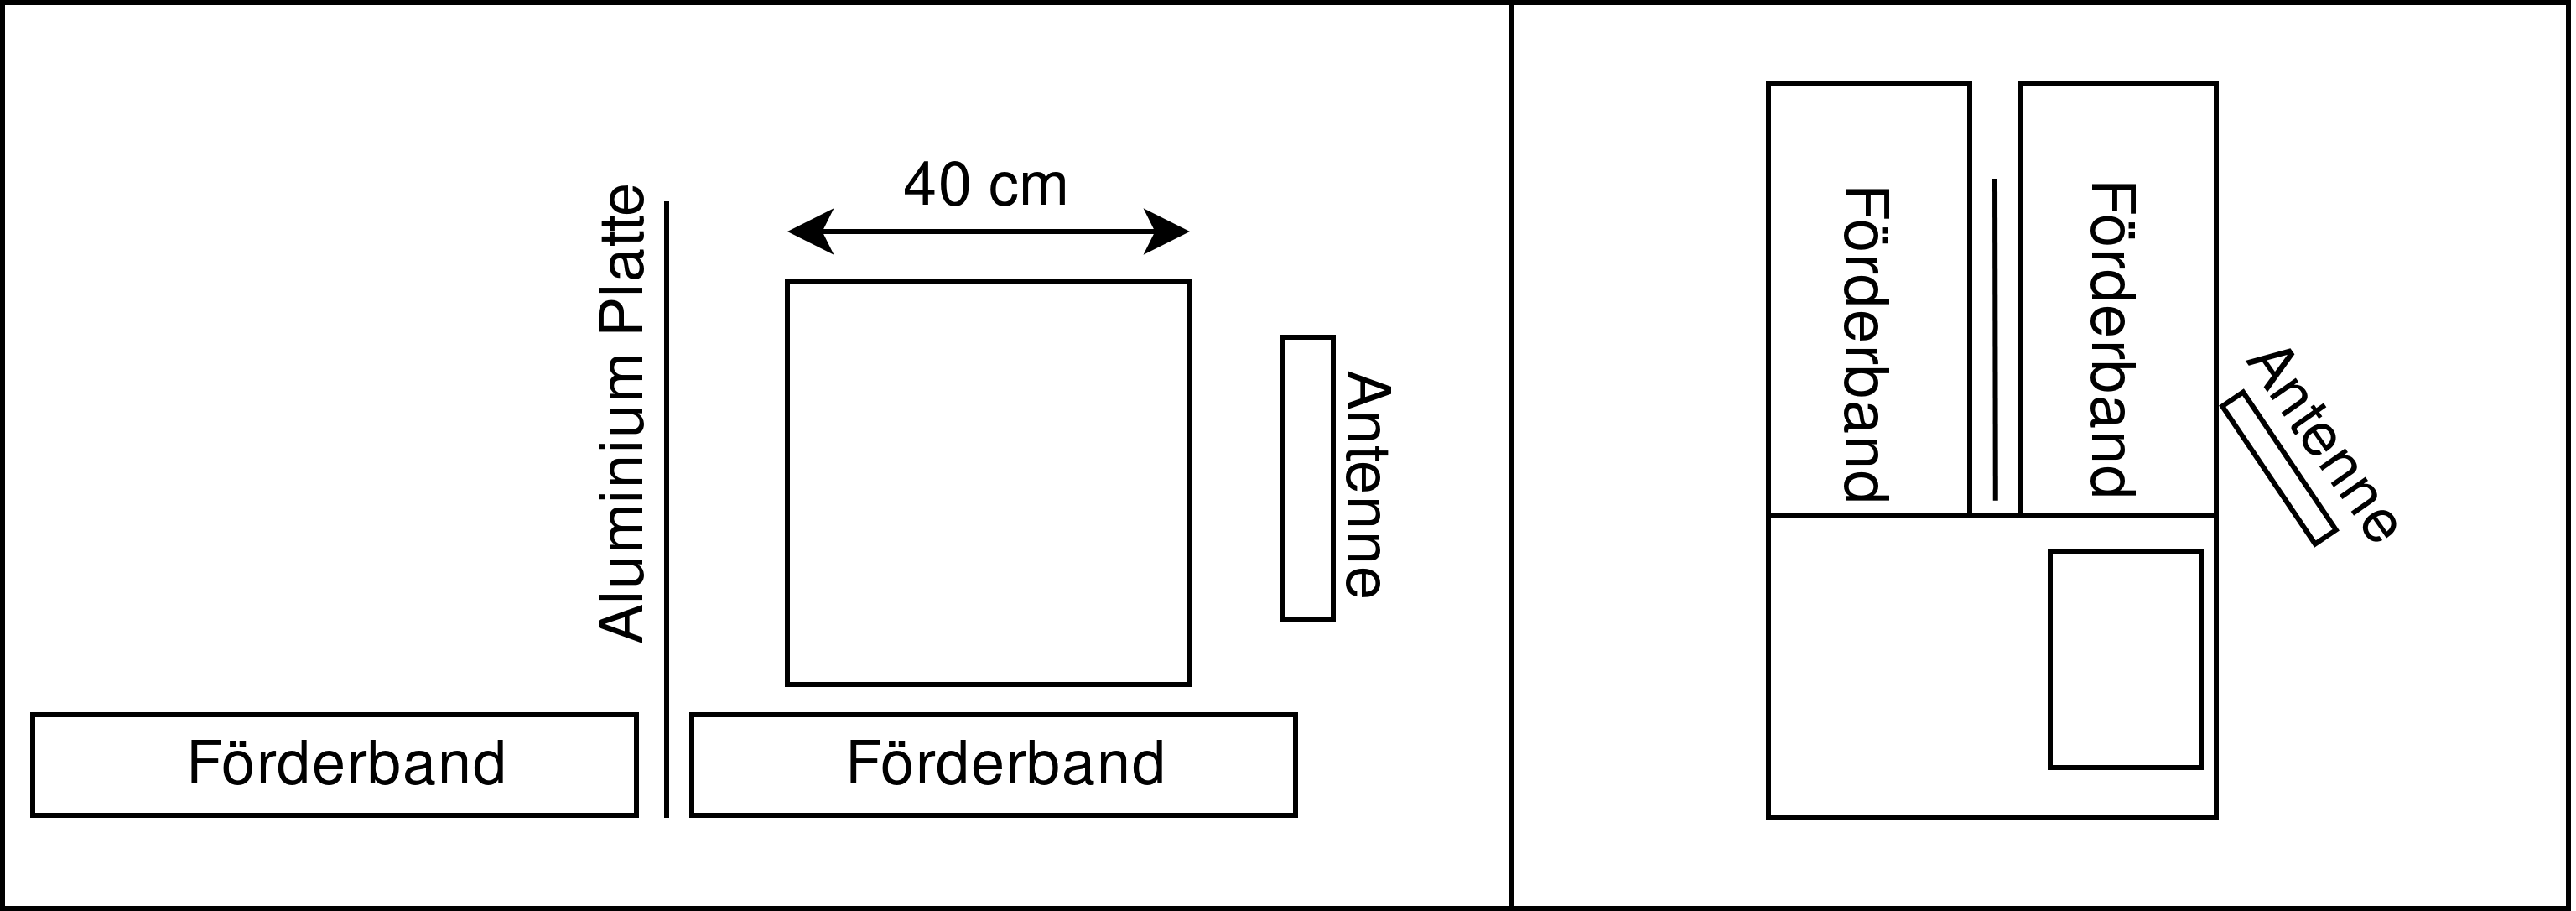
\includegraphics[keepaspectratio,width=.6\linewidth]{img/PositionierungAntennen}
	\caption{Positionierung der Antennen, links Schnitt, rechts Vogelperspektive}
	\label{fig:antenneSchraeg}
\end{figure}

Herr Baumann fügte noch an, dass bei Feig in der Hardware ein Embedded Linux System verwendet wird, welche es zulässt, dass direkt auf der Hardware programmiert wird und es keinen weiteren Computer wie ein RaspberryPi benötigt. Herr Wicki erklärte nochmals kurz an, dass beim Bulk Reading von RFID die Tags mittels Maske angesprochen werden, entspricht die Maske einem Tag, würde dieser antworten. Antworten mehrere Tags wird eine Kollision erkannt, und die Maske wird nochmals genauer definiert. Bei Feig könnte durch die Möglichkeit der Programmierung direkt auf der Hardware der Einsatz von mehreren Antennen optimiert werden, insofern als das eine bereits abgesuchte Maske bei der nächsten Antenne nicht nochmals komplett abgesucht werden muss. Herr Wicki fügte zudem noch an, dass dies bei der Jetzigen Hardware nicht möglich sei.
Weiter fügte Herr Wicki noch an, dass der Vorteil eines europäischen Herstellers darin liegt, dass dieser schneller und besser kontaktiert werden kann, und bei Problemen auch ein Besuch Vorort stattfinden könnte.
Herr Märki wies noch darauf hin, dass es bereits Tunnelantennen gegeben haben soll, diese jedoch, bedingt durch negative Resultate, nicht zum Einsatz kamen.
Herr Wicki antwortete noch mit der Aussage, dass beim Schreiben der Machbarkeitsstudie bestehende Lösungen bereits gesucht wurden und es keine gegeben hat. Es gab Lösungen, welche die Behälter zu identifizieren vermochten, nicht jedoch deren Inhalt. Herr Baumann fügte noch an, dass es lediglich eine ähnliche Lösung gibt, mit den Gates, welche bei Bibliotheken zu Verwendung kommen, diese jedoch auch nicht für solche Mengen wie in den Behältern der Speicherbibliothek anzutreffen sind.

Herr Baumann fuhr mit der Beschreibung der Machbarkeitsstudie fort. So erklärte er, dass zuerst die technische Beschreibung des Projektes vorzufinden ist, sowie auch das allgemeine Umfeld des Projekts. Zudem führt die Machbarkeitsstudie auf, dass keine Fördergelder vonseiten des Staates für dieses Projekt beantragt werden können. Anschliessend ist in der Machbarkeitsstudie der Entwicklungsplan beschrieben, welcher das Vorgehen für eine weitere Bachelorarbeit beschreibt. Dieser Anschaffungsplan wurde gemäss Herr Baumann in vier Aufgabenteile unterteilt. Herr Baumann fügt an, dass es für die Umsetzung zudem extrem wichtig sei, die Hardware bereits in der ersten dieser vier Phasen zu bestellen, damit diese auch zeitlich korrekt eintrifft. Anschliessend folgt in der Machbarkeitsstudie der Investitionsplan, welcher die Gesamtkosten für die Umsetzung dieses Projektes auflistet. Herr Baumann fügte an, dass vonseiten Stöcklin wahrscheinlich noch kleine Anpassungen vorgenommen werden müssen und daher deren Anpassungen auf 10'000 Franken geschätzt. Herr Wicki fügte bezüglich der 10'000 Franken noch an, dass diese wahrscheinlich soviel verlangen werden, um die Spezifikationen für das Automatische Ausschleusen zusammenzutragen und dem nachfolgenden Projektteam zu übergeben. Herr Märki fügte anschliessend noch an, dass das Budget von ca. 10'000 nicht genügend sein wird. Herr Wicki entgegnete, dass dieses Budget lediglich so tief geschätzt wurde, da Stöcklin bereits in der Lage ist Behälter auszuschleusen und dies nun nur noch mit allen Spezifikationen an das Folgeteam mitgeteilt werden muss und höchstwahrscheinlich keine teuren Softwareanpassungen anfallen werden. Herr Baumann fügte anschliessend noch hinzu, dass die Bindung zu Stöcklin gross ist, da sofern diese nicht in der Lage seien dem Team eine Schnittstelle zur Verfügung zu stellen, der gesamte Prozess des Ausschleusens nicht mehr realisierbar wäre. Herr Märki meinte noch, dass notfalls ein Drehlicht auch in Frage käme. Herr Wicki entgegnete, dass dies sicherlich möglich wäre, der optimale Fall jedoch die Integration in bestehende Prozesse wäre.

Herr Baumann meinte, das Projektteam wäre sehr froh um Rückmeldung bezüglich der Machbarkeitsstudie und ob diese etwa dem Entspräche, was Herr Märki sich vorgestellt habe. Er meinte zudem, dass Anpassungen bezüglich der Machbarkeitsstudie im kommenden Sprint angegangen werden, dementsprechend die Rückmeldung möglichst zeitnah erfolgen sollte.
Zudem wies er Herr Märki darauf hin, dass das Konzept Nummer Zwei nochmals etwas überarbeitet werden soll.
Herr Wicki fasste zusammen, dass im folgenden Sprint noch verschiedene Aufgaben zu erledigen sind. Es handelt sich dabei um die Anpassungen/Abgleich des Konzeptes gemäss der Machbarkeitsstudie, Anpassungen der Machbarkeitsstudie gemäss dem Feedback von Herr Märki, Fortsetzung der BDA, da diese bedingt durch den Zeitdruck etwas vernachlässigt wurde, zuletzt soll noch eine Referenzimplementation implementiert werden, welche vor Ort getestet werden kann.

Weiter fragte Herr Wicki Herr Märki ob dieser dem Team ein Datenbankauszug geben könnte, welcher reale Daten enthält. Herr Märki meinte, dass es ein Problem gäbe, dass das Team nicht weiss, was durchfliesst. Herr Wicki entgegnete, dass in einem ersten Schritt dies nicht von Bedeutung sei und es sich vielmehr um das korrekte verbinden und auslesen aus der Datenbank handle. Herr Märki meinte, er könne eine Tabelle erstellen, welche genau die zwei benötigten Felder enthält und diese dem Projektteam als Auszug zukommen zu lassen. Herr Märki fügte noch an, dass es nicht ratsam wäre in das Datenbankschema zu schauen, da dieses sehr komplex sei, daher schlage er vor, auf dem Datenbankserver eine View zu erstellen, welche genau die nötigen Informationen zusammenträgt. Herr Märki fragte noch nach, was dann mit diesen Daten gemacht werden würde. Herr Baumann antwortete, dass in Zusammenspiel mit einem Testbehälter, welcher Exemplare enthält, ein Testlauf gestartet werden kann. Herr Märki fragte noch nach, wie dann der Behälter identifiziert werden würde. Herr Baumann antwortete mit der Aussage, dass der Behälter über die Rückbeziehung der Mehrzahl der Tags erfolgen könne. Herr Wicki sagte anschliessend, dass es sinnvoll wäre die geschriebene Referenzimplementation noch vor Ort zu testen. Herr Baumann und Herr Märki stimmten dieser Aussage zu. Herr Baumann sagte, dass das Testen vor Ort zu Beginn des übernächsten Sprints zeitlich gut passen würde.

Herr Baumann rekapitulierte nochmals, dass das Team gerne vor Ort die Referenzimplementation mit Beginn des Sprintes 08 testen wollen, dafür ist es notwendig die Referenzimplementation in dem nächsten Sprint abzuschliessen. Weiter wird in diesem Sprint noch die Machbarkeitsstudie angepasst gemäs Rückmeldungen, sowie das Konzept angepasst.

\chapter{Anforderungen}
Herr Wicki begann zu erklären, dass mit Beginn des Projektes einige Voraussetzung für die kommende Referenzimplementation erstellt wurden, durch die Unklarheiten jedoch teilweise sehr offen formuliert wurden. Die erste Anforderung betreffe die Kommunikation mit der Datenbank. Herr Märki meinte, dass es für den Test nichts bringe mit der originalen Datenbank zu kommunizieren. Herr Wicki entgegnete, dass es trotzdem sinnvoll ist, mit der korrekten Datenbank Server Instanz kommunizieren zu können, auch wenn es sich bei dieser um einen, mit dem Auszug erzeugten, lokale Testdatenbank handle. Weiter meinte Herr Wicki, dass er diese Anforderungen so ergänzen würde, dass auch eine eigens gehostete Datenbank Server Instanz als Erfüllungskriterium hinzugefügt wird. Herr Märki akzeptierte dies.
Herr Baumann stellte anschliessend noch die Frage, wie die Antennen im Raum montiert werden können. Herr Wicki schlug vor, dass, bedingt durch den Umstand, dass Objekte am Boden deponiert werden, eine Vorrichtung ähnlich wie in Abbildung \ref{fig:montagevorrichtung} vom Projektteam erbaut werden soll. Herr Märki bestätigte, dass eine solche Vorrichtung auf den Boden gestellt werden kann.
\begin{figure}[htb]
	\centering
	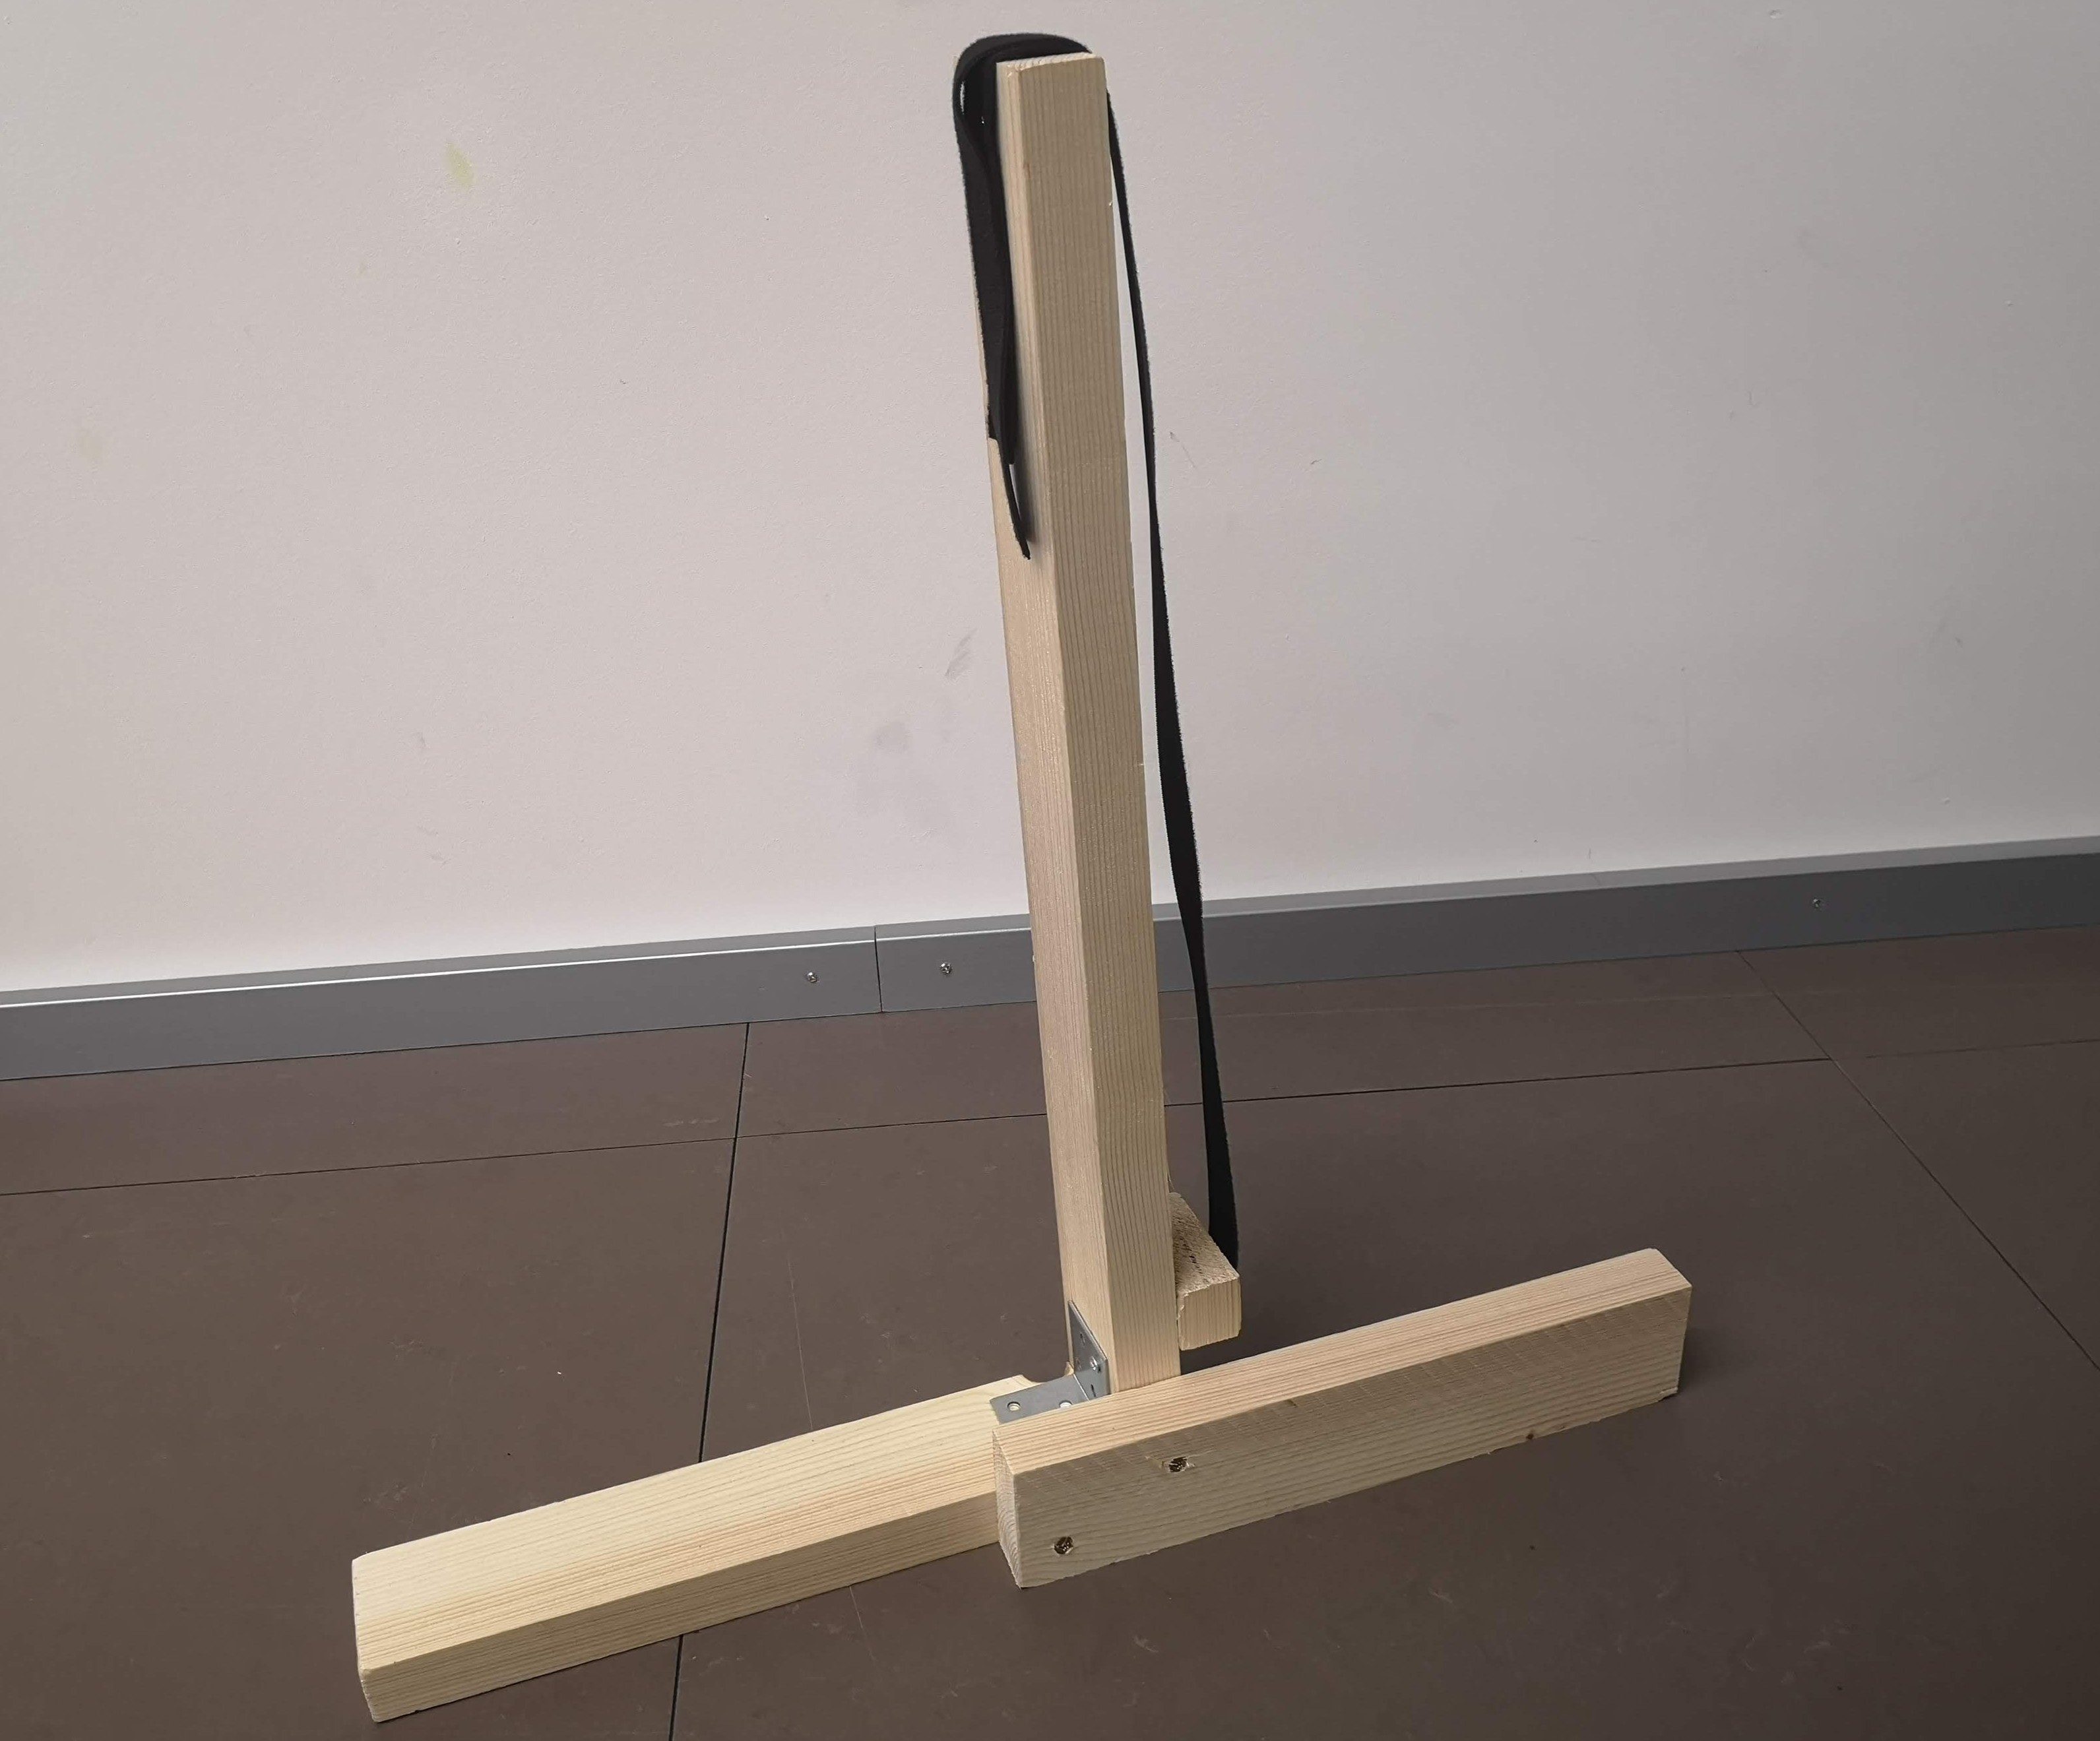
\includegraphics[keepaspectratio,width=.7\linewidth]{img/Montagevorrichtung}
	\caption{Montagevorrichtung für Versuche}
	\label{fig:montagevorrichtung}
\end{figure}
Herr Märki stellte noch die Frage, ob eine Oder 2 Antennen zum Einsatz kämen, da das Lesen mit der angewinkelten Antenne ihn doch noch sehr interessant dünkt. Herr Wicki meinte, dass für die Referenzimplementation nur eine Antenne verwendet wird, da nicht genug Zeit bestünde, eine gute Logik zu implementieren für das Wechseln der Antennen. Für den Test würde die Antenne einfach an beiden Positionen nacheinander manuell positioniert werden und so ausprobiert werden.
Herr Wicki forderte, dass dem Projektteam bekannt gegeben wird, wie hoch die Anlage ist. Herr Märki erklärte sich einverstanden dies dem Projektteam möglichst bald mitzuteilen.

Herr Wicki fasste zusammen, dass die Datenbank höhere Priorität habe wie die Höhenangabe. Die Höhenangabe soll bis zum 24.05.2019 Geliefert werden. Die Datenbank bis zum 17.05.2019. Herr Märki bestätigte die Fristen.

Herr Märki hinterfragte die gewählten Antennenpositionen. Herr Wicki begründete die Wahl neben dem Band damit, dass zwischen den Förderbändern nicht genügend Platz vorhanden ist, um die Antenne gut zu positionieren. Herr Märki entgegnete, dass es für den Test allenfalls auch Sinn ergibt, lediglich ein Holzbrett zwischen den Förderbändern zu Platzieren und die Antenne daraufzustellen. Herr Wicki entgegnete, dass dies für die Tests sicherlich möglich wäre, bedingt durch die angewinkelte Antenne, trotzdem eine Halterungsvorrichtung für diese erbaut werden müsste. Herr Wicki meinte, dass die Abschirmung weggelassen werden könnte, da für den Versuch jeweils nur einen Behälter getestet werden würde. Herr Märki entgegnete, dass es trotzdem sinnvoll wäre diese Abschirmung einzubauen, da es für Ihn sehr interessant ist, die Referenzimplementation unter Vollast auszuprobieren. Herr Wicki und Herr Baumann sind damit einverstanden.

Herr Märki fragte nochmals bezüglich der Antennenposition der angewinkelten Antenne nach, da ihm die diese Position noch nicht vollends zufriedenstellte. Herr Wicki schlug als Alternative vor, die Antenne am unteren Ende der Förderbänder zu positionieren (siehe Abbildung \ref{fig:neueAntennenposition}). Er wies jedoch darauf hin, dass mit der momentan verfügbaren Hardware von Hyientech diese Position als unmöglich erachtet wird, da die maximal Reichweite 60cm beträgt, und der Behälter bereits eine Länge von 60cm aufweist. Herr Wicki schlug deshalb vor, dass für das Konzept, bei welchem die Hardware von Feig verwendet werden soll diese Anpassungen gemacht werden, für den Test mit der Referenzimplementation jedoch trotzdem die Antenne angewinkelt platziert wird, da bei dieser Position der Behälter an der Antenne vorbeifährt und somit nicht 60cm gelesen werden muss. Herr Märki war mit dem Vorschlag einverstanden, wies jedoch noch auf die Position hin, bei welchem der Behälter in den Lift gefahren wird. Diese Position wurde jedoch von Herr Wicki und Herr Baumann als eher ungünstig ausgewiesen, da zu diesem Zeitpunkt das Ausschleusen nicht mehr möglich wäre.
\begin{figure}[htb]
	\centering
	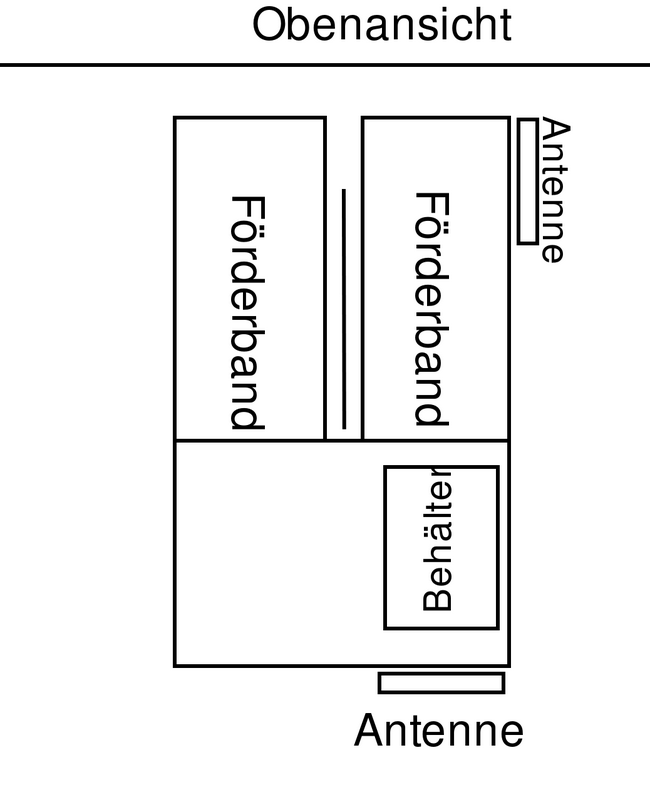
\includegraphics[keepaspectratio,width=.6\linewidth]{img/AntennenPositionNeu}
	\caption{Neue Positionierung am ende des Förderbandes}
	\label{fig:neueAntennenposition}
\end{figure}

Herr Baumann erklärte, dass die gemachten Fotos während des Kickoff Meetings teilweise zu wenig waren, um den gesamtem Überblick über die Anlage zu erhalten. Herr Märki erwiderte, dass er sonst noch Bildmaterial in Form eines Videos des nun zu verwendenden Abschnittes zur Verfügung stellt.

Herr Baumann fasste nochmals kurz zusammen, dass das Projektteam froh wäre die Höhe der Förderbänder und ein Foto oder Video der Eckpartie möglichst zeitnah zu erhalten.

Herr Wicki brachte nochmals die Anpassungen der Anforderung mit der Datenbank zu Sprache, bei welcher es nun genügt, dass eine eigene Datenbankinstanz verwendet wird. Herr Märki bestätigte dies für den Testlauf mit der Referenzimplementation. Herr Wicki fuhr mit der Anforderung fort, welche sagte, dass alle Tags lesbar sind. Grund dafür war gemäss Herr Wicki, dass nicht alle mit Tags ausgestatteten Exemplare technisch auch lesbar sind. Herr Wicki würde diese gerne anpassen, dass es neu heisst, dass alle Tags, welche auch technisch auslesbar sind, ausgelesen werden können. Herr Märki stimmte dem zu, da es ohne diese Anpassung nicht erfüllbar wäre.

Herr Märki merkte noch an, dass für ihn sehr interessant wäre, zu wissen, ob es möglich wäre einen einzelnen Tag anzufragen und ob dieser noch Lesbar wäre, auch bei gestapelten Tags. Herr Wicki antwortete, dass dies technisch nicht möglich ist, da das Bulk Reading im Prinzip gleich funktioniere wie ein Einzellesen. Es würde lediglich die Maske bereits bis zum letzten Bit definiert sein. Herr Wicki meinte, dass es gemäss seinem momentanen Wissen, keinen Unterschied mache, ob ein Tag spezifisch angesprochen wird oder über den Bulk Reading Modus. Gemäss den angaben von Herrn Wicki funktioniert es bei beiden gleich also, wenn es beim einen nicht funktioniert, so wird es beim zweiten auch nicht funktionieren. Herr Wicki bot trotzdem an diesen Versuch noch durchzuführen. Herr Märki erklärte sich einverstanden mit dem Angebot.

Herr Wicki fuhr mit der Nächsten Anforderung fort, welche besagte, dass einem User in belibiger Form die Nachricht einer gefunden Anomalie mitteilen kann. Gemäss Herr Wicki soll diese Anforderungen nun so angepasst werden, dass dem User über ein Konsolenfenster die Anomalie mitgeteilt werden soll. Weiter soll die Anforderung noch so angepasst werden, dass die Nachricht der Anomalie in einem Logdatei gespeichert wird. Herr Märki akzeptierte die vorgeschlagenen Änderungen.

Herr Wicki fragte noch an, ob die Anforderungen, bezüglich derselben Lesegenauigkeit bei einer Störfaktoren-bereinigten Umgebung wie bei den Versuchen, entfernt werden kann, da diese Anforderungen eher unsauber formuliert wurde. Herr Märki entgegnete, dass diese Anforderungen nicht entfernt werden solle, sondern eher so umgeschrieben werde, dass ein Artefakt entsteht, welches die Versuche mit den Resultaten der Referenzimplementation verifiziert. Herr Wicki und Herr Baumann haben dieser Umformulierung zugestimmt.
Herr Baumann fügte noch an, dass ein weiterer Versuch definiert wird, welcher die Versuche, welche bereits unter Laborbedingungen durchgeführt wurde, unter Realbedingungen durchführt. Herr Märki erklärte sich auch einverstanden mit dieser Anpassung merkte jedoch noch an, dass dem Projektteam nicht bekannt ist, welche Exemplare mit Tags ausgestattet sind.

\section{Tag-ID nicht gleich Exemplar-ID}
\label{result:noSingleTagReachable}
Herr Wicki fragte anschliessend, ob in der Datenbank nicht die Exemplare mit den Tag-IDs gespeichert werden, zumindest bei den Exemplaren, welche über einen Tag verfügen. Herr Märki erwiderte, dass die Datenbank keine Tag-ID speichert, sondern lediglich die Exemplar ID, welche nicht mit der Tag-ID übereinstimmt.

Herr Wicki wies darauf hin, dass unter diesen Umständen es nicht möglich ist nach einem Einzelexemplar zu suchen, da die Tag-ID der Applikation nicht bekannt ist. Herr Märki erwiderte, dass die Tag-ID und die Exemplar ID identisch seien. Herr Wicki wies darauf hin, dass die Tag-ID weltweit einmalig sei und auf einem Tag weitere Informationen gespeichert werden. Daraus leitete er ab, dass sich wohl die Exemplar-ID auf dem Tag befinde und somit eben eine Einzelexemplarsuche nicht Realisierbar ist. Herr Wicki wiederholte, dass es sehr unwahrscheinlich ist, dass eine Einzelexemplarsuche machbar ist, da die Tags die Exemplar ID wahrscheinlich gespeichert haben und somit die Tag-ID, welche bei der Einzelexemplarsuche bekannt sein muss nicht vorhanden ist. Herr Märki wie auch Herr Jud bestätigten, dass es wohl wahrscheinlicher sei, dass die Exemplar-ID auf den Tags gespeichert wird. Herr Wicki fragte noch nach, ob die Barcodes nach bekannt werden der Tags gedruckt werden. Herr Märki erwiderte, dass dies nicht der Fall sei.

Herr Wicki meinte, dass bedingt durch diese neue Tatsache, nur noch ein Bulk Reading gemacht werden kann, da wie bereits erwähnt für eine Einzelexemplarsuche die Tag-ID noch bekannt sein müsste. Herr Jud brachte noch die Idee ein, dass mit der Zeit eine solche Beziehung der Tag-ID mit der Exemplar-ID erstellt werden könnte. Jedoch meinte er auch, dass dies jedoch eher ungünstig für diese Situation ist, da diese erst über die Zeit erbaut werden kann.

Herr Wicki fragte, ob Herr Märki weiss in welchem Bereich die Exemplar-ID gespeichert ist. Herr Märki war nicht in der Lage dies zu beantworten. Herr Wicki schlug vor, dass das Projektteam den Lesebereich ausfindig zu machen unter der Verwendung von realen Exemplaren, welche in der ZHB in Rotkreuz vorhanden sind. Herr Märki war mit diesem Vorschlag einverstanden. Weiter nahm Herr Wicki dieses Lesen der Exemplar-ID als neue Anforderung auf. Herr Märki akzeptierte diese neue Anforderung.

Herr Märki fragte, ob die Tag-ID Überschreibbar ist. Herr Baumann antwortete, dass diese ID einmalig weltweit ist und diese ID beginnt stets mit der Herstellernummer.

\chapter{Rekapitulation der Entscheidungen}
Herr Wicki rekapitulierte das Meeting und listete die vom Projektteam gewünschten Artefakte nochmals auf. Dabei handelte es sich um den Datenbankauszug, das Foto/Video der Eckpartie, Höhe der Förderbänder und die Rückmeldung bezüglich der Machbarkeitsstudie. Herr Wicki verpflichtete sich, diese liste am Nachmittag Herrn Märki noch zukommen zu lassen. Herr Baumann fügte noch an, dass sich das Projektteam verpflichtet, einen Termin um den 27.05.2019 bis 29.05.2019 für die Referenzimplementation zu erstellen.  Herr Wicki verpflichtete sich noch die Anforderungen, wie auch die Machbarkeitsstudie digital an Herr Märki zukommen zu lassen.

\end{document}
